%%%%%%%%%%%%%%%%%%%%%%%%%%%%%%%%%%%%%%%%%%%%%%%%%%%%%%%%%%%%%%%%%%%%%%%%%%%%%%%
% Chapter 'Adsorption - Water - zeotype pellet AQSOA-Z01'
%%%%%%%%%%%%%%%%%%%%%%%%%%%%%%%%%%%%%%%%%%%%%%%%%%%%%%%%%%%%%%%%%%%%%%%%%%%%%%%
\subsection{Zeotype pellet AQSOA-Z01}
%
%%%%%%%%%%%%%%%%%%%%%%%%%%%%%%%%%%%%%%%%%%%%%%%%%%%%%%%%%%%%%%%%%%%%%%%%%%%%%%%
%%%%%%%%%%%%%%%%%%%%%%%%%%%%%%%%%%%%%%%%%%%%%%%%%%%%%%%%%%%%%%%%%%%%%%%%%%%%%%%
\subsubsection{DubininAstakhov - ID 1}
%
\begin{tabular}[l]{|lp{11.5cm}|}
\hline
\addlinespace

\textbf{Sorbent:} & zeotype pellet \\
\textbf{Subtype:} & AQSOA-Z01 \\
\textbf{Refrigerant:} & Water \\
\textbf{Equation:} & DubininAstakhov \\
\textbf{ID:} & 1 \\
\textbf{Reference:} & Wei Benjamin Teo, How; Chakraborty, Anutosh; Fan, Wu (2017): Improved adsorption characteristics data for AQSOA types zeolites and water systems under static and dynamic conditions. In: Microporous and Mesoporous Materials 242, S. 109–117. DOI: 10.1016/j.micromeso.2017.01.015. \\
\textbf{Comment:} & None \\

\addlinespace
\hline
\end{tabular}
\newline

\textbf{Properties of sorbent:}
\newline
%
\begin{longtable}[l]{lll}
\toprule
\addlinespace
\textbf{Property} & \textbf{Unit} & \textbf{Value} \\
\addlinespace
\midrule
\endhead
\bottomrule
\endfoot
\bottomrule
\endlastfoot
\addlinespace

Diameter of pore & \si{\milli\meter} & 0.0000074\\
Surface area & \si{\square\meter\per\gram} & 130-250\\
Pore volume & \si{\milli\cubic\meter\per\gram} & 0.071\\

\addlinespace\end{longtable}

\textbf{Equation and parameters:}
\newline
%
Loading $w$ in $\si{\kilogram\per\kilogram}$ is calculated depending on pressure $p$ in $\si{\pascal}$, temperature $T$ in $\si{\kelvin}$, and vapor pressure $p_\mathrm{sat}$ in $\si{\pascal}$ by:
%
\begin{equation*}
\begin{split}
w &=& \begin{cases} W \rho_\mathrm{sat}^{\mathrm{liq}} & \quad \text{if flag} \geq 0 \\ W & \quad \text{else} \end{cases} & \quad\text{, and} \\
W &=& W_0 \exp \left( - \left( \nicefrac{A}{E} \right) ^{n} \right) & \quad\text{, and} \\
A &=& R T \ln \left( \nicefrac{p_\mathrm{sat}}{p} \right) & \quad\text{.} \\
\end{split}
\end{equation*}
%
The parameters of the equation are:
%
\begin{longtable}[l]{lll|lll}
\toprule
\addlinespace
\textbf{Par.} & \textbf{Unit} & \textbf{Value} &	\textbf{Par.} & \textbf{Unit} & \textbf{Value} \\
\addlinespace
\midrule
\endhead

\bottomrule
\endfoot
\bottomrule
\endlastfoot
\addlinespace

flag & - & -1.000000000e+00 & $n$ & - & 5.000000000e+00 \\
$E$ & $\si{\joule\per\mole}$ & 4.000000000e+03 & $W_0$ & $\si{\kilogram\per\kilogram}$ & 2.100000000e-01 \\

\addlinespace\end{longtable}

\textbf{Validity:}
\newline
Equation is approximately valid for $476.7 \si{\pascal} \leq p \leq 17942.6 \si{\pascal}$,  $298.0 \si{\kelvin} \leq T \leq 333.0 \si{\kelvin}$, and $0.000788 \si{\kilogram\per\kilogram} \leq w \leq 0.218824 \si{\kilogram\per\kilogram}$.
\newline

\textbf{Visualization:}
%
\begin{figure}[!htp]
{\noindent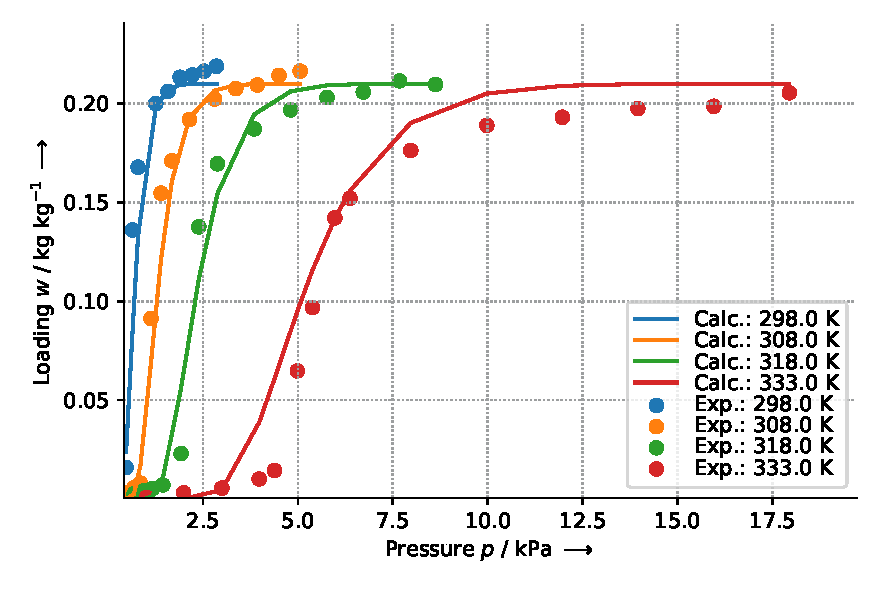
\includegraphics[height=10cm, keepaspectratio]{figs/ads/ads_Water_zeotype_pellet_AQSOA-Z01_DubininAstakhov_1.pdf}}
\end{figure}
%

To generate the figure, the following refrigerant functions were selected:
\begin{itemize}
\item Vapor pressure: VaporPressure\_EoS1 - ID 1
\item Saturated liquid density: SaturatedLiquidDensity\_EoS1 - ID 1
\end{itemize}

The uncertainity of the experimental data is:
\begin{itemize}
\item Data source $\,\to\,$ Data was taken from figure
\item Temperature, absolute, in $\si{\kelvin}$ $\,\to\,$ 0.15
\end{itemize}

The mean absolute percentage error (MAPE) between the experimental and calculated data results in 38.42\%.
\FloatBarrier
\newpage
%%%%%%%%%%%%%%%%%%%%%%%%%%%%%%%%%%%%%%%%%%%%%%%%%%%%%%%%%%%%%%%%%%%%%%%%%%%%%%%
%%%%%%%%%%%%%%%%%%%%%%%%%%%%%%%%%%%%%%%%%%%%%%%%%%%%%%%%%%%%%%%%%%%%%%%%%%%%%%%
\subsubsection{DubininAstakhov - ID 2}
%
\begin{tabular}[l]{|lp{11.5cm}|}
\hline
\addlinespace

\textbf{Sorbent:} & zeotype pellet \\
\textbf{Subtype:} & AQSOA-Z01 \\
\textbf{Refrigerant:} & Water \\
\textbf{Equation:} & DubininAstakhov \\
\textbf{ID:} & 2 \\
\textbf{Reference:} & Kayal, Sibnath; Baichuan, Sun; Saha, Bidyut Baran (2016): Adsorption characteristics of AQSOA zeolites and water for adsorption chillers. In: International Journal of Heat and Mass Transfer 92, S. 1120–1127. DOI: 10.1016/j.ijheatmasstransfer.2015.09.060. \\
\textbf{Comment:} & None \\

\addlinespace
\hline
\end{tabular}
\newline

\textbf{Properties of sorbent:}
\newline
%
\begin{longtable}[l]{lll}
\toprule
\addlinespace
\textbf{Property} & \textbf{Unit} & \textbf{Value} \\
\addlinespace
\midrule
\endhead
\bottomrule
\endfoot
\bottomrule
\endlastfoot
\addlinespace

Diameter of pore & \si{\milli\meter} & 0.0000074\\
Surface area & \si{\square\meter\per\gram} & 132\\
Pore volume & \si{\milli\cubic\meter\per\gram} & 0.087\\

\addlinespace\end{longtable}

\textbf{Equation and parameters:}
\newline
%
Loading $w$ in $\si{\kilogram\per\kilogram}$ is calculated depending on pressure $p$ in $\si{\pascal}$, temperature $T$ in $\si{\kelvin}$, and vapor pressure $p_\mathrm{sat}$ in $\si{\pascal}$ by:
%
\begin{equation*}
\begin{split}
w &=& \begin{cases} W \rho_\mathrm{sat}^{\mathrm{liq}} & \quad \text{if flag} \geq 0 \\ W & \quad \text{else} \end{cases} & \quad\text{, and} \\
W &=& W_0 \exp \left( - \left( \nicefrac{A}{E} \right) ^{n} \right) & \quad\text{, and} \\
A &=& R T \ln \left( \nicefrac{p_\mathrm{sat}}{p} \right) & \quad\text{.} \\
\end{split}
\end{equation*}
%
The parameters of the equation are:
%
\begin{longtable}[l]{lll|lll}
\toprule
\addlinespace
\textbf{Par.} & \textbf{Unit} & \textbf{Value} &	\textbf{Par.} & \textbf{Unit} & \textbf{Value} \\
\addlinespace
\midrule
\endhead

\bottomrule
\endfoot
\bottomrule
\endlastfoot
\addlinespace

flag & - & -1.000000000e+00 & $n$ & - & 5.000000000e+00 \\
$E$ & $\si{\joule\per\mole}$ & 4.000000000e+03 & $W_0$ & $\si{\kilogram\per\kilogram}$ & 2.100000000e-01 \\

\addlinespace\end{longtable}

\textbf{Validity:}
\newline
Equation is approximately valid for $127.0 \si{\pascal} \leq p \leq 9334.3 \si{\pascal}$,  $298.0 \si{\kelvin} \leq T \leq 338.0 \si{\kelvin}$, and $0.001131 \si{\kilogram\per\kilogram} \leq w \leq 0.212104 \si{\kilogram\per\kilogram}$.
\newline

\textbf{Visualization:}
%
\begin{figure}[!htp]
{\noindent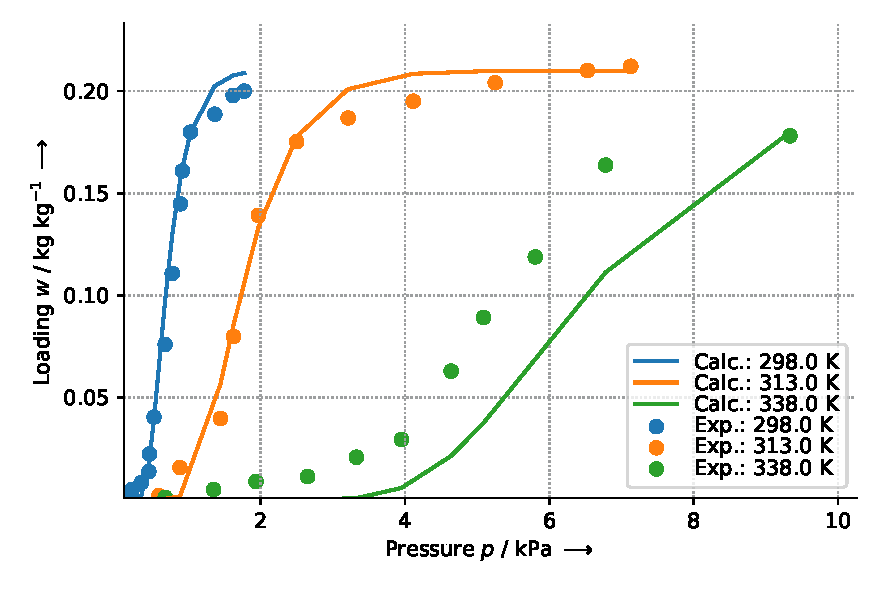
\includegraphics[height=10cm, keepaspectratio]{figs/ads/ads_Water_zeotype_pellet_AQSOA-Z01_DubininAstakhov_2.pdf}}
\end{figure}
%

To generate the figure, the following refrigerant functions were selected:
\begin{itemize}
\item Vapor pressure: VaporPressure\_EoS1 - ID 1
\item Saturated liquid density: SaturatedLiquidDensity\_EoS1 - ID 1
\end{itemize}

The uncertainity of the experimental data is:
\begin{itemize}
\item Data source $\,\to\,$ Data was taken from figure
\item Temperature, absolute, in $\si{\kelvin}$ $\,\to\,$ 0.01
\end{itemize}

The mean absolute percentage error (MAPE) between the experimental and calculated data results in 39.7\%.
\FloatBarrier
\newpage
%%%%%%%%%%%%%%%%%%%%%%%%%%%%%%%%%%%%%%%%%%%%%%%%%%%%%%%%%%%%%%%%%%%%%%%%%%%%%%%
